\documentclass[../../main]{subfiles}
\begin{document}

\subsection{Recommendations}
\label{ss:final-recommendations}

The recommendation section is the most important of the whole app considering the social- and context- aware implications.
Its purpose is to recommend places to the users of the application, both when they enter inside a \textit{geofence} and after a certain amount of time.
Recommendations are given as the result of the prediction classifier inside the recommendation model part of the server (see \hyperref[ss:recommendation-model]{Section 2.5}), which can output the best result for those given arguments. 
Places (that is, \textit{pois}) to recommend are not only searched between all the user's \textit{pois} but also between all the public ones owned by the user's friends.
When a place is found, the server sends a push notification to the user's device and, if the user taps on it, the detailed view of that \textit{poi} is shown.
In this scenario, the user is also asked to rate the recommendation, asking whether they are satisfied of the recommendation or if they wanted some other place of another category.\\
Some explicative pictures are shown below:
\begin{figure}[H]
    \centering
    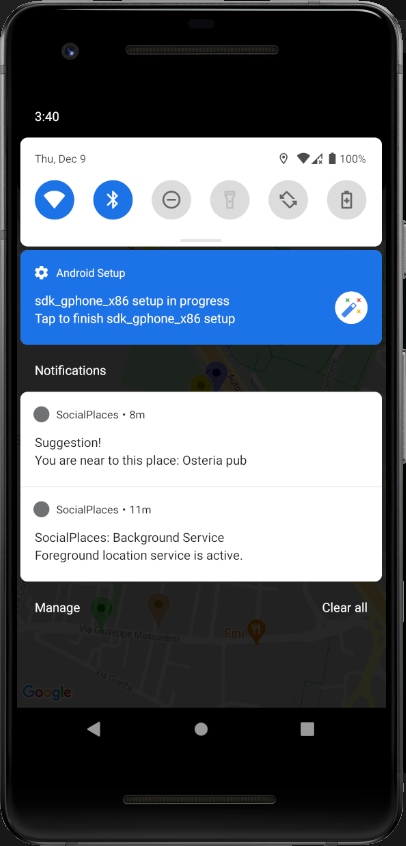
\includegraphics[width=0.4\textwidth]{images/app/notification/recommendation/recommendation_request}
    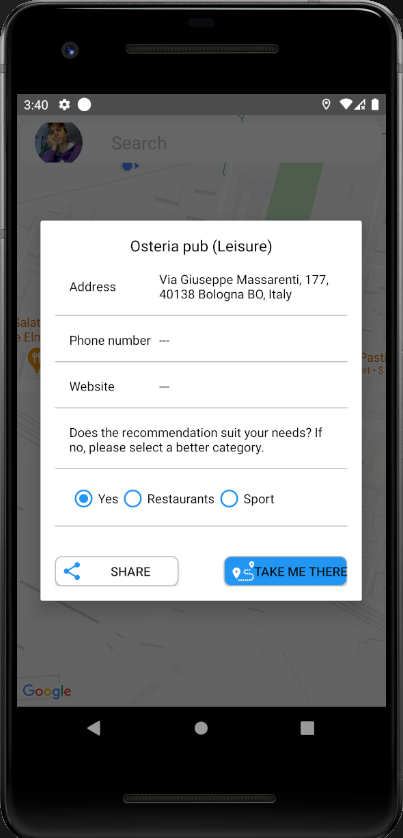
\includegraphics[width=0.4\textwidth]{images/app/notification/recommendation/user_feedback}
    \caption{On the left, the notification of a recommended place. On the right, the dialog for requesting the user's feedback on the recommendation which was just received.}
\end{figure}
\noindent
When the user closes the feedback's dialog, a new API call is sent to the backend in order to retrain the model.
When the model has retrained, a notification is sent with the new accuracy.
\begin{figure}[H]
    \centering
    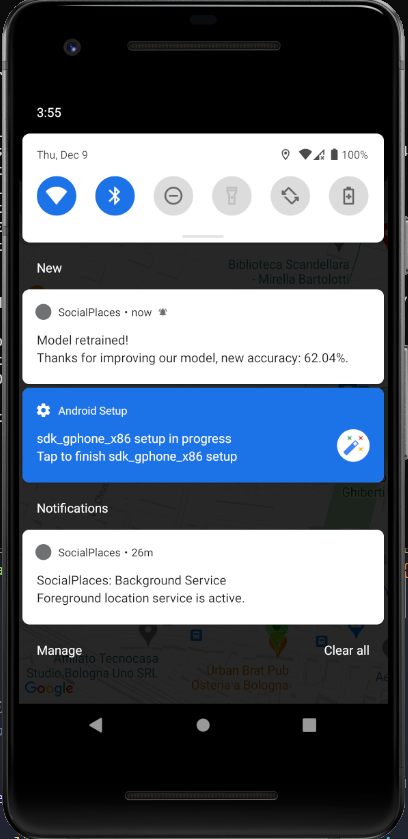
\includegraphics[width=0.4\textwidth]{images/app/notification/recommendation/new_accuracy}
    \caption{Model retrained notification.}
\end{figure}

\end{document}